%-- einleitung

\section{Projektumsetzung}
In diesem Abschnitt wird beschrieben, wie das Konzept umgesetzt wurde.
Es wird erläutert, für welche Programmteile welche Programmiersprachen eingesetzt werden. Darüber hinaus wird der Einsatz von Fremdbibliotheken aufgezeigt.
Anschließend wird mithilfe von  Programmcode-Ausschnitten die Implementierung der Genetischen Algorithmen erklärt.

\subsection{Programmiersprachen}
Durch die Trennung von Frontend und der Bibliothek ergeben sich für diese beiden Programmteile unterschiedliche Anforderungen an die Programmiersprache.\\
Die Bibliothek setzt die Genetischen Algorithmen um, die während einer Simulation mehrere tausend Berechnungen durchführt. Für diesen Zweck wurde sich für die Programmiersprache C++ entschieden.
Dabei handelt es sich um eine maschinennahe Sprache mit hohen Ausführungsgeschwindigkeiten. Allerdings ist die Entwicklung mit C++ sehr zeitaufwendig. Dadurch, dass es sich bei der Bibliothek um den zeitkritischen Teil des Projektes handelt, 
wurde sich trotz des hohen Aufwands für diese Programmiersprache entschieden.\\
Das Frontend hingegen soll lediglich die Verwendung der Bibliothek demonstrieren. In diesem Fall steht eine hohe Entwicklungsgeschwindigkeit im Vordergrund und deshalb wurde sich für Python als Frontend-Programmiersprache entschieden. 
Diese interpretierte Sprache ist im Vergleich zu C++ langsamer \cite{benchmarks}, ermöglicht aber eine schnellere und unkompliziertere Entwicklung.

\subsection{Frameworks und Bibliotheken}
Eine Übersicht über die verwendeten Bibliotheken ist in Tabelle \ref{tab:bibs} zu sehen.\\
Zur Entwicklung der Bibliothek für die Genetischen Algorithmen war ein Testsystem notwendig. Mit automatisierten Test wird sichergestellt, dass entwickelter Code die angedachten Aufgaben korrekt erfüllt.
Für diesen Zweck wurde die C++ Bibliothek Catch2 eingesetzt. Bei Catch2 handelt es sich um eine sogenannte Single-Header-Library. Das bedeutet, dass der gesamte Bibliothekscode in einer Datei zu finden ist.
Dadurch war eine sehr einfache Einbindung in das Projekt möglich. Catch2 läuft unter der Boost-Software-License, was eine freie Nutzung der Bibliothek ermöglicht.\\
Des Weiteren wurde eine Bibliothek zum Visualisieren von Simulationsergebnissen eingesetzt. Dazu wurde die sehr beliebte Matplotlib verwendet. Diese ermöglicht das einfache erstellen von Graphen in Python aber auch C++.
In diesem Projekt wurde Matplotlib nur auf der Python-Seite verwendet. Die Bibliothek läuft unter der Matplotlib-License, bei der es sich um eine Open-Source-Lizens handelt.\\
Damit ein Python Programm überhaupt C++ Code ausführen kann, ist es notwenig Schnittstellen von C++ zu Python bereitzustellen. Dafür wurde das Python-Modul der Boost-Bibliothek verwendet. Mit diesem war eine sehr schnelle Entwicklung von Schnittstellen möglich.
Auch die Boost-Bibliothek läuft unter der Boost-Software-Lizence und ist dadurch für eine kostenlose Nutzung freigegeben.
\begin{table}
\caption{Verwendeten Bibliotheken}
\begin{tabular}{|l|l|l|l|}
 Name & Version & Anwendung & Lizenz \\ 
\hline
 Catch2 & 2.13 & Unit-Tests der Library & Boost Software License \cite{catch2} \\  
 Matplotlib & 3.2 & Visualisierung der Experimente & Matplotlib License \cite{matplotlib} \\
 Boost & 1.7 & Schnittstelle zwischen C++ und Python & Boost Software License  \cite{boost}   
\end{tabular}
\label{tab:bibs}
\end{table}

\subsection{Individuen und Populationen}
Wie in der Systemmodellierung \ref{fig:systemmodellierung} zu sehen war, verarbeiten die Genetischen Algorithmen Individuen und Populationen. Aus diesem Grund wurden diese beiden Objekttypen als Klasse implementiert. Das dazugehörige Klassendiagramm ist in Abbildung \ref{fig:klassendiagramm} zu sehen.
Die Individuen speichern dabei die Chromosome als ganzzahlige Liste. In dieser Liste sind die Routeninformationen gespeichert. Es wurde sich dafür entschieden, die Route als eine Liste von nacheinander besuchten Stadtindezes zu implementieren. Die Startstadt ist allerdings kein Teil dieser Liste, weil sich diese bei den Verarbeitungsschritten nicht verändern soll.
Der Vorteil dieser Codierung ist eine leichte Überprüfbarkeit der TSP-Vorgabe, dass jede Stadt nur einmal besucht werden darf. Es muss lediglich berechnet werden, dass jede Stadt, außer der Startstadt, innerhalb der Liste genau einmal vorkommt. Diese Validierungsfunktionalität ist in der Methode \texttt{is\_valid} des Individuums implementiert.
Hätte man sich für eine binäre Codierung entschieden, bei der die Bitposition angibt, welche Verbindungen besucht wurden, dann wäre eine solche Überprüfung deutlich komplizierter \cite[S. 271-271]{schoeneburg}.\\
Ein Individuum benötigt für die Verarbeitung innerhalb der Genetischen Algorithmen eine Fitness- und eine Bewertungsfunktion. Die Bewertungsfunktion berechnet, wie nah ein Individuum an einem optimalen Individuum liegt und die Fitnessfunktion entspricht der Wahrscheinlichkeit, als Elternindividuum ausgewählt zu werden.
Ein Individuum bekommt seine Fitness- und Bewertungsfunktion bei der Objekterstellung übergeben. Somit wird ermöglicht diese Funktionen sehr schnell auszutauschen. Die Funktionen \texttt{fitness} und \texttt{rating} des Individuums verwenden anschließend lediglich diese injizierten Funktionen.\\
Eine Menge an Individuen bildet eine Population. Eine Populationen wird dazu eingesetzt unkompliziert mit vielen Individuen zu arbeiten. Dazu bietet diese Klasse die Funktionalität die Fitness aller enthaltenen Individuen zu berechnen, das fitteste und unfitteste Individuum zurückzugeben und die Menge an Individuen zu aktualisieren.
Darüber hinaus speichert die Population die Startstadt und die Distanzdaten. Diese sind zur Berechnung der Fitness und Bewertung der Individuen notwendig.
\begin{figure}[H]
\centering
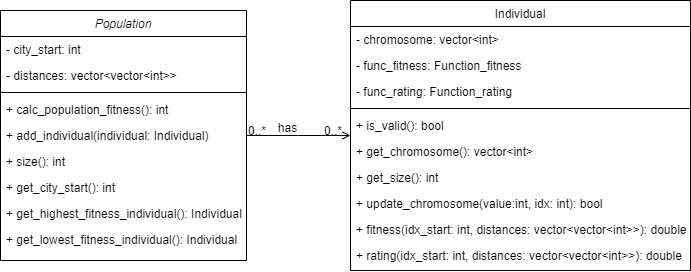
\includegraphics[width=1\textwidth]{img/Vortrag/uml.png}
\caption{Klassendiagramm Individuum und Population}
\label{fig:klassendiagramm}
\end{figure}


\subsection{Bewertungs und Fitnessfunktion}
In Listing \ref{lst:rating} ist eine Bewertungsfunktion zu sehen, die in diesem Projekt verwendet wurde. Diese berechnet die Bewertung eines Chromosoms mit Hilfe einer Distanzmatrix. In Zeile 4 wird die Distanz von der Startstadt zur ersten Stadt innerhalb des Chromosoms bestimmt. Anschließend werden von Zeile 5 bis 9 alle Distanzen innerhalb des Chromosoms hinzugerechnet. Als letztes wird in Teile 10 die Verbindung der letzten Stadt im Chromosom zur Startstadt addiert. Somit ist die Bewertung die Gesamtdistanz der Route und die funktionale Anforderung 3FA ist erfüllt. Diese Distanz soll innerhalb des Verfahrens minimiert werden.\\
In Listing \ref{lst:fitness} ist die Fitnessfunktion zu sehen, die in diesem Projekt verwendet wurde. Diese negiert lediglich die berechneten Bewertungen der Individuen. Damit wird erreicht, dass ein Individuum mit einer niedrigen Gesamtdistanz als fitter angesehen wird als ein Individuum mit hoher Gesamtdistanz.

\begin{minipage}{\linewidth}
\begin{lstlisting}[caption={Beispiel einer Bewertungsfunktion}, firstnumber=1, captionpos=b, label=lst:rating]
double func_rating(int idx_start, vector<int> chromosome, vector<vector<int>> distances){
	int city_a, city_b;
	int rating = 0;
	costs += get_distance(idx_start, chromosome.at(0), distances);
	for (unsigned int i = 0; i < chromosome.size() - 1; ++i) {
		city_a = chromosome.at(i);
		city_b = chromosome.at(i + 1);
		rating += get_distance(city_a, city_b, distances);
	}
	rating += get_distance(chromosome.at(chromosome.size() - 1), idx_start, distances);
	return rating;
}
\end{lstlisting}
\end{minipage}
\begin{minipage}{\linewidth}
\begin{lstlisting}[caption={Beispiel einer Fitnessfunktion}, firstnumber=1, captionpos=b, label=lst:fitness]
double func_fitness(double rating){
	return -rating;
}
\end{lstlisting}
\end{minipage}
\subsection{Marriage-Algorithmus}
Bei den Genetischen Algorithmen entspricht die Hochzeit der Wahl von Elternindivuen aus einer Population. Diese Eltern werden anschließend verwendet um Nachkommen zu generieren. 
Die Auswahl ist dabei zufällig, jedoch sollen Individuen mit einer höheren Fitness eine höhere Wahrscheinlichkeit haben ausgewählt zu werden. 
Mit der Fitnessfunktion ergeben sich allerdings noch negative Fitnesswerte. Um diese Werte verwenden zu können, werden die Fitnesswerte jeweils mit der Fitness des unfittesten Individuums der Population subtrahiert. Eine beispielhafte Umrechnung ist in Tabelle \ref{tab:roulette} zu sehen. Das Individuum 5 entspricht dem unfittesten invididuum. \\
Im Codebeispiel \ref{lst:marriage} ist eine Umsetzung eines solchen Hochzeit-Verfahrens zu sehen. Das beschriebene Verfahren nennt sich Roulette-Marriage \cite[S. 204]{schoeneburg}. Bei diesem Algorithmus wird zuerst ein Roulette-Rad aufgebaut, bei dem jedes Individuum einen Bereich im Rad repräsentiert.
So auch zu sehen in den Zeilen 4 bis 7. Je höher das Delta der Fitness, desto größer ist der Bereich. In den Teilen 8 und 9 werden zwei Kugeln generiert, die in das Roulette-Rad geworfen werden. In den Zeilen 12 bis 20 wird berechnet in welche Bereiche die Kugeln gelandet sind. Anschließend werden die Indizes der 
gewählten Elternindividuen zurückgegeben.

\begin{minipage}{\linewidth}
\begin{lstlisting}[caption={Marriage-Roulette Algorithmus}, firstnumber=1, captionpos=b, label=lst:marriage]
pair<int, int> marriage_roulette_reversed(Population &population) {
	pair<int, int> pair = make_pair(-1, -1);
	int sum = 0;
	int worst_fitness_of_population = (int) population.get_lowest_fitness_individual().get_last_calculates_fitness();
	for (auto &it : population.get_individuals()) {
		sum += (int) it.get_last_calculates_fitness() - worst_fitness_of_population;
	}
	int value_p1 = random(sum);
	int value_p2 = random(sum);

	int value = 0;
	for (unsigned int current_idx = 0; current_idx < population.size(); ++current_idx) {
		value += (int) population.get_individuals().at(current_idx).get_last_calculates_fitness() - worst_fitness_of_population;
		if (value_p1 <= value && pair.first < 0) {
			pair.first = current_idx;
		}
		if (value_p2 <= value && pair.second < 0) {
			pair.second = current_idx;
		}
	}
	return pair;
}
\end{lstlisting}
\end{minipage}
\begin{table}[H]
\center
\caption{Umrechnung der Fitness-Werte}
\begin{tabular}{|l|l|l|}
 Individuum & Fitness & Delta \\ 
\hline
 1 & -1180 & 820 \\  
 2 & -1680 & 320 \\  
 3 & -1860 & 140 \\  
 4 & -1880 & 120 \\  
 5 & -2000 & 0 \\  
\end{tabular}
\label{tab:roulette}
\end{table}

\subsection{Crossover-Algorithmen}
Die Crossover-Verfahren sind ein wichtiger Bestandteil der Genetischen Algorithmen. Sie definieren, wie aus zwei Elterninviduen Nachkommen generiert werden.
In diesem Projekt wurde eine ganze Reihe von Crossover-Verfahren umgesetzt. Die Algorithmen wurden mit einhaltlicher Signatur implementiert. Sie bekommen zwei Elternindividuen und zwei Kinderindividuen übergeben.
Die Informationen aus den Elternindividuen werden verarbeitet und anschließend in die Kinderindividuen geschrieben.

\subsubsection{Partially-Matched-Crossover}
Das Partially-Matched-Crossover \cite[S. 273]{schoeneburg} ist ein Verfahren, das dazu neigt die absoluten Elementpositionen zu erhalten. Eine Umsetzung ist in Listing \ref{lst:pmx} zu sehen. Zum leichteren Verständnis wird das Verfahren an einem Beispiel in Tabelle \ref{tab:pmx} gezeigt.
Im Schritt 0 werden zwei zufällige Intervallgrenzen für die Chromosome der Eltern gewählt. Dieser Schritt ist im Codebeispiel in der Zeile 3 zu sehen.
Im Schritt 1 werden die Daten außerhalb des Intervalls des Elternindividuums 1 in das Kind 1 und innerhalb des Intervalls in das Kind 2 geschrieben. Für das Elternindividuum 2 wird genau umgekehrt vorgegangen. Das beschriebene Vorgehen ist in den Zeilen 5 bis 13 zu sehen.
Die so generierten Kindinviduen sind allerdings nicht immer valide. So kommt zum Beispiel im Kindindividuum 1 die Stadt 4 mehrmals vor. Aus diesem Grund muss eine Korrektur durchgeführt werden.
Bei dieser Korrektur werden die Kindindividuen durchlaufen und kontrolliert, welche Städte zweimal vorkommen. Eins dieser Vorkommen muss immer im Intervall liegen. Im Beispiel ist das im Kindindividuum 1 die Stadt 4 mit dem Index 1. Anschließend wird untersucht, welche Stadt im Elternindividuum 1 an der Position 1 liegt. Im Beispiel ist das die Stadt 2. Nun wird die Stadt 4 des Kindindividuums 1, außerhalb des Intervalls, mit der Stadt 2 überschrieben. Somit ergibt sich ein korrigiertes Individuum. Für das Kindindividuum 2 wird genauso vorgegangen, nur das Chromosom mit dem Elternindividuum 2 verglichen wird.
Zur besseren Lesbarkeit übernimmt die Korrektur eine Hilfsfunktion in Zeile 15 und 16.
\begin{table}[H]
\centering
\caption{Beispiel für das Partially-Matched-Crossover}
\begin{tabularx}{0.5\textwidth}{l|l|l}
Schritt & Individuum & Chromosom\\
\hline
\multirow{2}{*}{Schritt 0}
		& Elter 1 & 1 | 2 3 | 4 5\\
		&  Elter 2 & 5 | 4 3 | 2 1\\
\hline
\multirow{2}{*}{Schritt 1}
		& Kind 1 &  1 | 4 3 | 4 5\\
		&  Kind 2 & 5 | 2 3 | 2 1\\
\hline
\multirow{2}{*}{Schritt 2}
		& Kind 1 &  1 | 4 3 | 2 5\\
		&  Kind 2 & 5 | 2 3 | 4 1\\
\end{tabularx}
\label{tab:pmx}
\end{table}

\begin{minipage}{\linewidth}
\begin{lstlisting}[caption={Partially-Matched-Crossover}, firstnumber=1, captionpos=b, label=lst:pmx]
void partially_matched_crossover(Individual &p1, Individual &p2, Individual &c1, Individual &c2) { 
	int length = p1.get_size();
	int interval_border_left, interval_border_right = calc_two_random_interval_borders(length);

	for (int i = 0; i < length; ++i) {
		if (i < interval_border_left || i >= interval_border_right) {
			c1.update_chromosome(p1.get_chromosome().at(i), i);
			c2.update_chromosome(p2.get_chromosome().at(i), i);
		} else {
			c1.update_chromosome(p2.get_chromosome().at(i), i);
			c2.update_chromosome(p1.get_chromosome().at(i), i);
		}
	}

	duplicate_correction_pmx(p1, p2, c1);
	duplicate_correction_pmx(p2, p1, c2);
}
\end{lstlisting}
\end{minipage}
\subsubsection{Order-Crossover}
Das Vorgehen des Order-Crossover-Verfahrens \cite[S. 274]{schoeneburg} ist ähnlich zu dem Partially-Matched-Crossover-Verfahren, nur dass nun zuerst Duplikate korrigiert und anschließend Chromosome getauscht wird.
Eine Umsetzung ist im Codelisting \ref{lst:ox} zu sehen. In Tabelle \ref{tab:ox} ist ein Anwendungsbeispiel schrittweise aufgeführt. Im Schritt 0 werden zwei Intervallgrenzen gesetzt. Dies Codebeispiel wird das in Zeile 3 durchgeführt.
Im Schritt 1 werden die Elemente, die innerhalb des jeweils anderen Elternteils vorkommen, als Lücke X markiert. Dafür werden im Code in den Zeilen 5 bis 9 Mengen generiert, die dazu dienen zu speichern, welche Elemente innerhalb der Intervalle vorkommen.
Anschließend wird in den Zeilen 11 bis 12 die Lücke innerhalb der Kindindividuen gesetzt. Dazu wird innerhalb der Variablen \texttt{Cache} gespeichert, an welcher Stelle die Duplikate aufgetreten sind. Im Schritt 2 werden die Chromosome neu sortiert. Dabei wird an der linken Intervallgrenze gestartet und die Lücken in das Intervall verschoben. Die Umsortierung wird im Code in den Zeilen 13 und 14 durchgeführt. Um nun die Lücken korrekt zu verschieben, werden die \texttt{Caches}, die zuvor berechnet wurden, eingesetzt. In diesen ist gespeichert, wo die Dopplung auftrat und wo nun die Lücke platziert werden muss.
Nach der Umsortierung, kann der Tausch im Schritt 3 in den Zeilen 16 bis 23 durchgeführt werden.

\begin{table}[H]
\centering
\caption{Partially-Matched-Crossover}
\begin{tabularx}{0.5\textwidth}{l|l|l}
Schritt & Individuum & Chromosom\\
\hline
\multirow{2}{*}{Schritt 0}
		& Elter 1 & 1 | 2 3 | 4 5\\
		& Elter 2 & 5 | 4 3 | 2 1\\
\hline
\multirow{2}{*}{Schritt 1}
		& Kind 1 & 1 | 2 3 | X 5\\
		& Kind 2 & 5 | 4 3 | X 1\\
\hline
\multirow{2}{*}{Schritt 2}
		& Kind 1 & 2 | X 3 | 5 1\\
		& Kind 2 & 4 | X 3 | 1 5\\
\hline
\multirow{2}{*}{Schritt 3}
		& Kind 1 & 2 | 4 3 | 5 1\\
		& Kind 2 & 4 | 2 3 | 1 5\\
\end{tabularx}
\label{tab:ox}
\end{table}


\begin{minipage}{\linewidth}
\begin{lstlisting}[caption={Order-Crossover}, firstnumber=1, captionpos=b, label=lst:ox]
void order_crossover(Individual &p1, Individual &p2, Individual &c1, Individual &c2) {
	int length = p1.get_size();
	int interval_border_left, interval_border_right = calc_two_random_interval_borders(length);

	unordered_map<int, int> map_p1, map_p2;
	for (int i = interval_border_left; i < interval_border_right; ++i) {
		map_p1.insert(pair<int, int>(p1.get_chromosome().at(i), i));
		map_p2.insert(pair<int, int>(p2.get_chromosome().at(i), i));
	}
	vector<int> cache1, cache2;
	set_duplicate_flags(map_p2, c1, p1, cache1, interval_border_left, interval_border_right);
	set_duplicate_flags(map_p1, c2, p2, cache2, interval_border_left, interval_border_right);
	copy_values(c1, cache1, interval_border_left);
	copy_values(c2, cache2, interval_border_left);

	for (int j = interval_border_left; j < interval_border_right; ++j) {
		if (c1.get_chromosome().at(j) == DUPLICATE_FLAG) {
			c1.update_chromosome(p2.get_chromosome().at(j), j);
		}
		if (c2.get_chromosome().at(j) == DUPLICATE_FLAG) {
			c2.update_chromosome(p1.get_chromosome().at(j), j);
		}
	}
}
\end{lstlisting}
\end{minipage}
\subsubsection{One-Cycle-Crossover}
Bei den Cycle-Crossover-Verfahren \cite[S. 275]{schoeneburg} werden Wert-Zyklen zwischen den Chromosomen der beiden Elternindividuen gebildet, um einen Teil der Erbinformationen zu kreuzen, während die restlichen Informationen lediglich kopiert werden.
Um einen Wert-Zyklus zu bilden, wird an einer beliebigen Stelle im ersten Elternchromosom begonnen. An dieser Stelle werden die Werte beider Chromosome vermerkt. Der Wert des zweiten Elternchromosoms an dieser Stelle muss im ersten Chromosom gefunden werden und bestimmt somit das nächste Wert-Tupel des Zyklus. Ein Zyklus ist abgeschlossen, sobald eine Stelle doppelt betrachtet wird. Das Code-Listing \ref{lst:find_cycle} verdeutlicht die Vorgehensweise.

\begin{minipage}{\linewidth}
\begin{lstlisting}[caption={Zyklus finden}, firstnumber=1, captionpos=b, label=lst:find_cycle]
bool fill_empty_cycle_with_tuples(Cycle &cycle, int cycle_start_idx, Individual &p1, Individual &p2, std::vector<bool> &index_flags) {
    int idx = cycle_start_idx;
    do {
        index_flags.at(idx) = true;
        int v1 = p1.get_chromosome().at(idx);
        int v2 = p2.get_chromosome().at(idx);
        cycle.emplace_back(idx, v1, v2);
        idx = vector_find(p1.get_chromosome(), v2);
        if (idx == -1) {
            std::cerr
                    << "chromosome value of second parent cannot be found in first parent chromosome. chromosomes must consist of the same set of values."
                    << std::endl;
            return false;
        }
    } while (!index_flags.at(idx));
    return true;
}
\end{lstlisting}
\end{minipage}

Dieses Crossover-Verfahren funktioniert nur, wenn beide Elternchromosome aus der gleichen Wertmenge bestehen und innerhalb eines Chromosoms kein Wert doppelt vorkommt.
Stehen in beiden Chromosomen am gleichen Index die gleichen Werte, so entsteht dort ein Zyklus der Größe $1$. Solch ein Zyklus resultiert immer in einem Kopieren der Werte, da das Vertauschen zweier gleicher Werte redundant ist. Diese Zyklen können dazu führen, dass sich die Kinder nicht von den Eltern unterscheiden.
Das gleiche geschieht, wenn der gefundene Zyklus jedes Element der Eltern beinhaltet. Auch in diesem Fall wird lediglich eine Kopie der Eltern vorgenommen - ein Crossover bleibt aus.\\
Bei dem One-Cycle-Crossover wird lediglich ein Zyklus der Chromosome verwendet, um eine Kreuzung durchzuführen. Es wird ein Wert-Zyklus beginnend bei einem zufälligen Startindex gebildet. Dieser Zyklus dient der reinen Informationsweitergabe an die Kinder. Alle weiteren Stellen im Chromosom werden gekreuzt.
In Code-Listing \ref{lst:cxo} ist das beschriebene One-Cycle-Crossover-Verfahren umgesetzt.

\begin{minipage}{\linewidth}
\begin{lstlisting}[caption={One-Cycle-Crossover}, firstnumber=1, captionpos=b, label=lst:cxo]
void cycle_crossover_one_cycle(Individual &p1, Individual &p2, Individual &c1, Individual &c2) {
	vector<bool> index_flags(p1.get_size(), false);
	Cycle cycle;
	int cycle_start_idx = random(p1.get_size());
	fill_empty_cycle_with_tuples(cycle, cycle_start_idx, p1, p2, index_flags)
	int tupleCounter = 0;
	for (int i = 0; (unsigned int) i < index_flags.size(); ++i) {
		bool flag = index_flags.at(i);
		if (flag) {
			Tuple &t = cycle.at(tupleCounter);
			tupleCounter++;
			c1.update_chromosome(get<1>(t), get<0>(t));
			c2.update_chromosome(get<2>(t), get<0>(t));
		} else {
 			c1.update_chromosome(p2.get_chromosome().at(i), i);
			c2.update_chromosome(p1.get_chromosome().at(i), i);
		}
	}
}
\end{lstlisting}
\end{minipage}

\subsubsection{All-Cycles-Crossover}
Im Gegensatz zum One-Cycle-Crossover werden bei dem All-Cycles-Crossover-Verfahren alle Wert-Zyklen der Elternchromosome miteinbezogen.
Im Code-Listing \ref{lst:cxa} ist eine solche Umsetzung zu sehen. Bei dieser wurden die Zyklen in den Zeilen 4 bis der Reihe nach aufgebaut und anschließend in den Zeilen 12 bis 14 in der selben Reihenfolge durchlaufen. 
Das Auswahlverfahren der zu betrachtenden Zyklen kann aber auch per Zufall geschehen. Anschließend wird zuerst ein Zyklus kopiert, der nächste wird hingegen zur Kreuzung der Erbinformationen verwendet. Dieser Vorgang wird in den Zeilen 12 bis 24 solange wiederholt bis alle Zyklen durchlaufen sind.

\begin{minipage}{\linewidth}
\begin{lstlisting}[caption={All-Cycles-Crossover}, firstnumber=1, captionpos=b, label=lst:cxa]
void cycle_crossover_all_cycles(Individual &p1, Individual &p2, Individual &c1, Individual &c2) {
	vector<bool> index_flags(p1.get_size(), false);
	vector<Cycle> cycles;
	for (int cycle_start_idx = 0; cycle_start_idx < p1.get_size(); ++cycle_start_idx) {
		Cycle cycle;
		if (!index_flags.at(cycle_start_idx)) {
			fill_empty_cycle_with_tuples(cycle, cycle_start_idx, p1, p2, index_flags)
		}
		cycles.push_back(cycle);
		}
	}
	for (int i = 0; (unsigned int) i < cycles.size(); ++i) {
		bool cross_copy = i % 2 != 0;
		Cycle &cycle = cycles.at(i);
		for (Tuple &t : cycle) {
			if (cross_copy) {
				c1.update_chromosome(get<2>(t), get<0>(t));
				c2.update_chromosome(get<1>(t), get<0>(t));
			} else {
				c1.update_chromosome(get<1>(t), get<0>(t));	
 				c2.update_chromosome(get<2>(t), get<0>(t));
			}
		}
	}
}

\end{lstlisting}
\end{minipage}
\subsubsection{Edge-Recombination-Crossover}
Das Edge-Recombination-Crossover-Verfahren \cite[S. 276]{schoeneburg} ist ein kantenbasiertes Verfahren. Eine Umsetzung ist im Codelisting \ref{lst:erx} zu sehen. Für ein besseres Verständnis wird ein Beispiel in Tabelle \ref{tab:erx2} eingesetzt.\\
Für das Edge-Recombination-Crossover-Verfahren wird zu Beginn eine Kanten-Map generiert. In dieser Datenstruktur wird gespeichert, zwischen welchen Städten Verbindungen bestehen. Das wird im Code in Zeile 2 durchgeführt und generiert im Beispiel die Kanten-Map in Tabelle \ref{tab:em}.
Anschließend wird in Schritt 1 der Startpunkt der Kinderindividuen gewählt. Dieser ist entweder das erste Element des Elter 1 oder Elter 2. Im Folgenden wird nur die Erzeugung des Kind 1 betrachtet. Kind 2 wird nach demselben Verfahren, mit lediglich einem anderen Startpunkt, erzeugt.
Die Stadt 0 wir nun aus allen Verbindungslisten der Edge-Map gelöscht. Die Löschung ist in den Zeilen 12 bis 14 zu sehen. Anschließend wird geschaut, welche Stadt in der Verbindungsliste von Stadt 0 die wenigsten Verbindungen hat. Die Auswahl der Stadt mit der kleinsten Verbindungsliste ist in den Zeilen 18 bis 23 zu sehen. Diese Stadt ist die nächste Stadt, die in das Individuum eingetragen wird. Haben mehrere Städte die gleiche Anzahl an Verbindungen wird zufällig eine Stadt ausgewählt. In dem Beispiel hat die Stadt 4 die kleinste Anzahl an Verbindungen und wird somit ausgewählt, in das Kind gespeichert und als aktuelles Element betrachtet. Dieser Vorgang wird so lange wiederholt, bis alle Verbindungslisten leer sind.

\begin{table}[H]
\centering
\caption{Edge-Recombination-Crossover}
\begin{tabularx}{0.5\textwidth}{l|l|l}
Schritt & Individuum & Chromosom\\
\hline
\multirow{2}{*}{Schritt 0}
		& Elter 1 & 0 4 1 2 3\\
		& Elter 2 & 2 1 3 0 4\\
\hline
\multirow{2}{*}{Schritt 1}
		& Kind 1 & 0\\
		& Kind 2 & 2\\
\hline
\multirow{2}{*}{Schritt 2}
		& Kind 1 & 0 4 \\
		& Kind 2 & 2 1 \\
\hline
\multirow{2}{*}{Schritt 3}
		& Kind 1 & 0 4 1\\
		& Kind 2 & 2 1 4\\
\hline
\multirow{2}{*}{Schritt 4}
		& Kind 1 & 0 4 1 3\\
		& Kind 2 & 2 1 4 0\\
\hline
\multirow{2}{*}{Schritt 5}
		& Kind 1 & 0 4 1 3 2\\
		& Kind 2 & 2 1 4 0 3\\
\end{tabularx}
\label{tab:erx2}
\end{table}

\begin{table}[H]
\center
\caption{Edge-Map}
\begin{tabular}{l|l}
Stadt & Verbindungen \\
\hline
0 & 3 4\\
1 & 2 3 4\\
2 & 1 3\\
3 & 0 1 2\\
4 & 0 1\\
\end{tabular}
\label{tab:em}
\end{table}

\begin{minipage}{\linewidth}
\begin{lstlisting}[caption={Edge-Recombination-Crossover}, firstnumber=1, captionpos=b, label=lst:erx]
bool edge_recombination_crossover(Individual &p1, Individual &p2, Individual &c1, Individual &c2) {
	map<int, set<int>> edge_map = create_edge_map(p1, p2);
	edge_recombination(p1.get_chromosome().at(0),c1, edge_map);
	edge_recombination(p2.get_chromosome().at(0),c2, edge_map);
	return true;
}

void edge_recombination(int start, Individual &i, map<int, set<int>> edge_map) {
	int current = start;
	for (int idx = 0; idx < i.get_size() - 1; ++idx) {
		i.update_chromosome(current, idx);
		for (auto &it : edge_map) {
			it.second.erase(current);
		}
		int min_next_idx = -2;
		unsigned int min_next_count = numeric_limits<int>::max();

		for (int node : edge_map.at(current)) {
			if (edge_map.at(node).size() < min_next_count) {
				min_next_count = edge_map.at(node).size();
				min_next_idx = node;
			}
		}
		current = min_next_idx;
		if (idx == i.get_size() - 2) {
			i.update_chromosome(current, idx + 1);
		}
	}
}
\end{lstlisting}
\end{minipage}

\subsection{Mutations-Algorithmus}
Die Aufgabe des Mutations-Algorithmus ist es, neu generierte Kinderindividuen mit einer Mutationsrate zu mutieren.
In diesem Projekt wurde dazu der Delete-Shift-Mutationsalgorithmus \cite[S. 277]{schoeneburg} in Listing \ref{lst:mutation} eingesetzt. Dieser bekommt eine Mutationsrate und ein Individuum übergeben.
Anschließend wird in Zeile 2 mit zufällig entschieden, ob eine Mutation durchgeführt wird oder nicht. Wenn mutiert wird, werden in den Zeilen 4 und 5 zwei Intervallgrenzen berechnet, innerhalb derer die Mutation durchgeführt wird.
Bei der Delete-Shift-Mutation wird das Element an der linken Intervallgrenze gelöscht und alle Elemente innerhalb des Intervalls, rechts von dem gelöschten Element, um eine Position nach links verschoben. Dadurch entsteht eine Lücke an der rechten Intervallgrenze. An diese Stelle muss das gelöschte Element geschrieben werden. Anstelle des eigentlichen Löschens wurde sich im Codebeispiel in den Zeilen 7 bis 9 für ein hintereinander ausgeführtes tauschen der Elemente entschieden. Dieser Ansatz führt zu den gleichen Resultaten, ergibt aber besser lesbaren Programmcode.

\begin{minipage}{\linewidth}
\begin{lstlisting}[caption={Delete-Shift-Mutaions-Algorithmus}, firstnumber=1, captionpos=b, label=lst:mutation]
bool mutation_delete_shift(Individual &individual, int percentage) {
	bool mutate = rand(100)  < percentage;
	if (mutate) {
		int position_a = rand(individual.get_size() - 1);
		int position_b = rand(position_a + 1, individual.get_size());
 
		for (int i = position_a; i < position_b; i++) {
			swap_chromosome(individual.get_chromosome(), i, i + 1);
		}
	}
	return mutate;
}
\end{lstlisting}
\end{minipage}
\subsection{Selektions-Algorithmus}
Der Selektionsalgorithmus erstellt aus zwei übergebenen Populationen eine neue Population, die nur eine Auswahl der Individuen aus den übergebenen Populationen enthält.
In diesem Projekt wurde die Survivol-of-the-Fittest-Selektion \ref{lst:selektion} eingesetzt. Bei dieser besteht die neu entstandene Population aus den fittesten Individuen beider Populationen.
In den Zeilen 7 bis 11 werden die Individuen nach ihrer Fitness absteigend sortiert. Anschließend werden die sortierten Individuen in den Zeilen 14 bis 22 durchlaufen und die besten Individuen in eine neue Population geschrieben. Die neue Population wird in der Zeile 23 zurückgegeben.

\begin{minipage}{\linewidth}
\begin{lstlisting}[caption={Survival-Of-The-Fittest-Selektions-Algorithmus}, firstnumber=1, captionpos=b, label=lst:selektion]
Population selection_sotf(Population &p_old, Population &p_new) {
	int size = (int) p_old.size();
	p_old.calc_population_fitness();
	p_new.calc_population_fitness();
	Population result = Population(p_old.get_idx_start(), p_old.get_distances());

	vector<Individual> individuals_old = p_old.get_individuals();
	vector<Individual> individuals_new = p_new.get_individuals();

	sort(individuals_new.rbegin(), individuals_new.rend());
	sort(individuals_old.rbegin(), individuals_old.rend());
	int offset_old = 0;
	int offset_new = 0;
	for (int i = 0; i < size; ++i) {
		if (individuals_old.at(offset_old) < individuals_new.at(offset_new)) {
			result.add_individual(individuals_new.at(offset_new));
			offset_new++;
		} else {
			result.add_individual(individuals_old.at(offset_old));
 			offset_old++;
		}
	}
	return result;
}
\end{lstlisting}
\end{minipage}
\subsection{Simulator}
Der Simulator ist eine Klasse, die die einfache Bedienung der Genetischen Algorithmen ermöglichen soll. Dieser soll Einstellungsmöglichkeiten in seinem Konstruktor entgegennehmen, mit der eine Simulation durchgeführt wird. Das Klassendiagramm des implementierten Simulators ist in der Grafik \ref{fig:simulator} zu sehen. Neben dem Konstruktor enthält der Simulator noch eine Funktion \texttt{simulate}, die eine Generationsstufe ausführt. Innerhalb einer Generationsstufe werden die Genetischen Algorithmen in der korrekten Reihenfolge ausgeführt. Diese Funktion gibt die höchste Fitness, die niedrigste Fitness und eine durchschnittliche Fitness der Population zurück, die nach dem Generationsschritt vorliegen. Darüber hinaus kann mit der Funktion \texttt{best\_individual} das Chromosom des aktuell fittesten Individuums zurückgegeben werden.

\begin{figure}[H]
\centering
\includegraphics[width=0.6\textwidth]{img/Vortrag/simulator.png}
\caption{Klassendiagramm Simulator}
\label{fig:simulator}
\end{figure}

\subsection{Python-Schnittstelle}
Um eine C++ Bibliothek in Python verwenden zu können, müssen Schnittstellen bereitgestellt werden. Für diesen Zweck wurde die Boost-Python-Bibliothek eingesetzt. Diese ermöglicht das einfache und schnelle Erstellen solcher Schnittstellen. Im Listing \ref{lst:boostpython} ist ein Ausschnitt, der für dieses Projekt erstellten Schnittstelle, zu sehen. In der Zeile 1 wird ein Python-Modul erstellt. Dieses Modul kann anschließend in einem Python-Programm importiert werden. Sollen C++ spezifische Datenstrukturen zurückgegeben werden so sind Übersetzer einzusetzen. In der Zeile 3 ist ein solcher Übersetzer zu sehen, der C++ Tupels zu Python Listen übersetzt. In der Zeile 5 ist ein Beispiel für ein C++ Enum aufgeführt. Die Schnittstelle für den Simulator ist in den Zeilen 7 bis 14 definiert. Dabei wird mit dem Schlüsselwort \texttt{init} der Konstruktor angegeben und mit \texttt{def} alle weiteren Funktionen, die auf Pythonseite zur Verfügung stehen sollen. Da der Nutzer nur den Simulator für eine TSP-Simulation verwenden soll, waren keine Schnittstellen für die Genetischen Algorithmen notwendig.

\begin{minipage}{\linewidth}
\begin{lstlisting}[caption={C++ zu Python Schnittstelle}, firstnumber=1, captionpos=b, label=lst:boostpython]
BOOST_PYTHON_MODULE(Simulator_Wrapper)
{
	to_python_converter<tuple<int, int, int>, TupleToList<int> >();

	enum_<Selection_Algorithm>("Selection_Algorithm").value("SOTF", Selection_Algorithm::SOTF);

	class_<Simulator>("Simulator", init<
		string, string, string,
		int,int,int,int,
		Crossover_Algorithm, Marriage_Algorithm, Mutation_Algorithm, Selection_Algorithm>(
		))
 		.def("simulate", &Simulator::simulate)
		.def("finished", &Simulator::finished)
		.def("best_individual", &Simulator::best_individual);
}
\end{lstlisting}
\end{minipage}
\subsection{Testen}
Das Testen hat bei der Projektumsetzung eine besondere Rolle eingenommen. Ein automatisches Testsystem führt nicht nur zu Code mit weniger Fehlern, sondern hilft auch dabei zu verstehen, was sich ein Entwickler bei der Implementierung gedacht hat. Somit können Tests eine mangelhafte Dokumentation ausgleichen.\\
Für das schnelle Erstellen von Tests wurde die Catch2 Bibliothek eingesetzt. Diese überzeugte durch die einfache Bedienung und Projekteinbindung.
Mit Catch2 werden Szenarien definiert, die bestimmte Testfälle abdecken. So zu sehen in Codelisting \ref{lst:tests}. Innerhalb des \texttt{REQUIRE} werden die eigentlichen Kontrollen durchgeführt.
Für dieses Projekt wurden 26 Testszenarien definiert, die die Korrektheit von Implementierungen kontrollieren.
\begin{minipage}{\linewidth}
\begin{lstlisting}[caption={Unit-Tests}, firstnumber=1, captionpos=b, label=lst:tests]
SCENARIO("Test Individual initialization", "[Individual.cpp]")
{
	for (int i = 0; i < 100; ++i) {
		Individual individual = Individual(size, idx_start, nullptr, nullptr);
		vector<int> chromosome = individual.get_chromosome();
		REQUIRE(chromosome.size() == (unsigned int) size);
		REQUIRE(unique(chromosome.begin(), chromosome.end()) == chromosome.end());
	}
}
\end{lstlisting}
\end{minipage}
%--